\begin{exe}
    \ex Andrew hits Mathis.\hfill\textit{\footnotesize $4/15$ iterations, 2.63ms}
        \begin{xlist}
            % input string: "[.\node(top){S}; [.NP^1 [.N^1 Andrew ] ] [.VP [.V hits ] [.NP^2 [.N^2 Mathis ] ] ] ]"
            \ex \begin{tikzpicture}[baseline=(top.base)]
                    \Tree [.\node(top){S}; [.NP [.N Andrew ] ] [.VP [.V hits ] [.NP [.N Mathis ] ] ] ]
                \end{tikzpicture}
            \ex \begin{tikzpicture}[baseline=(top.base)]
                    \Tree [.\node(top){S\,^{{\color{darkgray}\mathtt{FA\shortleftarrow}}}_{{\color{gray}t}} }; [.NP\,^{{\color{darkgray}\mathtt{NN}}}_{{\color{gray}e}} [.N\,^{{\color{darkgray}\mathtt{NN}}}_{{\color{gray}e}} Andrew\,^{{\color{darkgray}\mathtt{TN_1}}}_{{\color{gray}e}} ] ] [.VP\,^{{\color{darkgray}\mathtt{FA\shortrightarrow}}}_{{\color{gray}\langle e,\, t\rangle}} [.V\,^{{\color{darkgray}\mathtt{NN}}}_{{\color{gray}\langle e,\, \langle e,\, t\rangle\rangle}} hits\,^{{\color{darkgray}\mathtt{TN_1}}}_{{\color{gray}\langle e,\, \langle e,\, t\rangle\rangle}} ] [.NP\,^{{\color{darkgray}\mathtt{NN}}}_{{\color{gray}e}} [.N\,^{{\color{darkgray}\mathtt{NN}}}_{{\color{gray}e}} Mathis\,^{{\color{darkgray}\mathtt{TN_1}}}_{{\color{gray}e}} ] ] ] ]
                \end{tikzpicture}
        \end{xlist}
    \end{exe}

\begin{exe}
    \ex Not tanzt.\hfill\textit{\footnotesize $7/15$ iterations, 1.49ms}
        \begin{xlist}
            % input string: "[.\node(top){A}; [.B not [.C [.D [.E [.F [.G tanzt ] ] ] ] [.Peter ] ] ] ]"
            \ex \begin{tikzpicture}[baseline=(top.base)]
                    \Tree [.\node(top){A}; [.B not [.C [.D [.E [.F [.G tanzt ] ] ] ] [.Peter ] ] ] ]
                \end{tikzpicture}
            \ex \begin{tikzpicture}[baseline=(top.base)]
                    \Tree [.\node(top){A\,^{{\color{darkgray}\mathtt{NN}}}_{{\color{gray}t}} }; [.B\,^{{\color{darkgray}\mathtt{FA\shortrightarrow}}}_{{\color{gray}t}} not\,^{{\color{darkgray}\mathtt{TN_1}}}_{{\color{gray}\langle t,\, t\rangle}} [.C\,^{{\color{darkgray}\mathtt{FA\shortrightarrow}}}_{{\color{gray}t}} [.D\,^{{\color{darkgray}\mathtt{NN}}}_{{\color{gray}\langle e,\, t\rangle}} [.E\,^{{\color{darkgray}\mathtt{NN}}}_{{\color{gray}\langle e,\, t\rangle}} [.F\,^{{\color{darkgray}\mathtt{NN}}}_{{\color{gray}\langle e,\, t\rangle}} [.G\,^{{\color{darkgray}\mathtt{NN}}}_{{\color{gray}\langle e,\, t\rangle}} tanzt\,^{{\color{darkgray}\mathtt{TN_1}}}_{{\color{gray}\langle e,\, t\rangle}} ] ] ] ] [.Peter\,^{{\color{darkgray}\mathtt{TN_1}}}_{{\color{gray}e}} ] ] ] ]
                \end{tikzpicture}
        \end{xlist}
    \end{exe}

\begin{exe}
    \ex Der große verschüchterte fliegende Wolf aus Twilight.\hfill\textit{\footnotesize $7/15$ iterations, 3.96ms}
        \begin{xlist}
            % input string: "[.\node(top){DP}; [.D der ] [.NP [.AP [.A große ] ] [.N$''''$ [.AP^2 [.A^2 verschüchterte ] ] [.N$'''$ [.AP^3 [.A^3 fliegende ] ] [.N$''$ [.N$'$ [.N Wolf ] ] [.PP [.P aus ] [.NP^2 [.N^2 Twilight ] ] ] ] ] ] ] ]"
            \ex 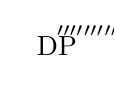
\begin{tikzpicture}[baseline=(top.base)]
                    \Tree [.\node(top){DP}; [.D der ] [.NP [.AP [.A große ] ] [.N$''''$ [.AP [.A verschüchterte ] ] [.N$'''$ [.AP [.A fliegende ] ] [.N$''$ [.N$'$ [.N Wolf ] ] [.PP [.P aus ] [.NP [.N Twilight ] ] ] ] ] ] ] ]
                \end{tikzpicture}
            \ex \begin{tikzpicture}[baseline=(top.base)]
                    \Tree [.\node(top){DP\,^{{\color{darkgray}\mathtt{FA\shortrightarrow}}}_{{\color{gray}e}} }; [.D\,^{{\color{darkgray}\mathtt{NN}}}_{{\color{gray}\langle \langle e,\, t\rangle,\, e\rangle}} der\,^{{\color{darkgray}\mathtt{TN_1}}}_{{\color{gray}\langle \langle e,\, t\rangle,\, e\rangle}} ] [.NP\,^{{\color{darkgray}\mathtt{PM}}}_{{\color{gray}\langle e,\, t\rangle}} [.AP\,^{{\color{darkgray}\mathtt{NN}}}_{{\color{gray}\langle e,\, t\rangle}} [.A\,^{{\color{darkgray}\mathtt{NN}}}_{{\color{gray}\langle e,\, t\rangle}} große\,^{{\color{darkgray}\mathtt{TN_1}}}_{{\color{gray}\langle e,\, t\rangle}} ] ] [.N$''''$\,^{{\color{darkgray}\mathtt{PM}}}_{{\color{gray}\langle e,\, t\rangle}} [.AP\,^{{\color{darkgray}\mathtt{NN}}}_{{\color{gray}\langle e,\, t\rangle}} [.A\,^{{\color{darkgray}\mathtt{NN}}}_{{\color{gray}\langle e,\, t\rangle}} verschüchterte\,^{{\color{darkgray}\mathtt{TN_1}}}_{{\color{gray}\langle e,\, t\rangle}} ] ] [.N$'''$\,^{{\color{darkgray}\mathtt{PM}}}_{{\color{gray}\langle e,\, t\rangle}} [.AP\,^{{\color{darkgray}\mathtt{NN}}}_{{\color{gray}\langle e,\, t\rangle}} [.A\,^{{\color{darkgray}\mathtt{NN}}}_{{\color{gray}\langle e,\, t\rangle}} fliegende\,^{{\color{darkgray}\mathtt{TN_1}}}_{{\color{gray}\langle e,\, t\rangle}} ] ] [.N$''$\,^{{\color{darkgray}\mathtt{PM}}}_{{\color{gray}\langle e,\, t\rangle}} [.N$'$\,^{{\color{darkgray}\mathtt{NN}}}_{{\color{gray}\langle e,\, t\rangle}} [.N\,^{{\color{darkgray}\mathtt{NN}}}_{{\color{gray}\langle e,\, t\rangle}} Wolf\,^{{\color{darkgray}\mathtt{TN_1}}}_{{\color{gray}\langle e,\, t\rangle}} ] ] [.PP\,^{{\color{darkgray}\mathtt{FA\shortrightarrow}}}_{{\color{gray}\langle e,\, t\rangle}} [.P\,^{{\color{darkgray}\mathtt{NN}}}_{{\color{gray}\langle e,\, \langle e,\, t\rangle\rangle}} aus\,^{{\color{darkgray}\mathtt{TN_1}}}_{{\color{gray}\langle e,\, \langle e,\, t\rangle\rangle}} ] [.NP\,^{{\color{darkgray}\mathtt{NN}}}_{{\color{gray}e}} [.N\,^{{\color{darkgray}\mathtt{NN}}}_{{\color{gray}e}} Twilight\,^{{\color{darkgray}\mathtt{TN_1}}}_{{\color{gray}e}} ] ] ] ] ] ] ] ]
                \end{tikzpicture}
        \end{xlist}
    \end{exe}

\begin{exe}
    \ex Andrew malt den Wolf und_{ind} die Blumen.\hfill\textit{\footnotesize $7/15$ iterations, 3.12ms}
        \begin{xlist}
            % input string: "[.\node(top){S}; [.NP [.N Andrew ] ] [.VP [.V malt ] [.CoordP [.DP^1 [.D^1 den ] [.NP^2 [.N^2 Wolf ] ] ] [.Coord$'$ [.Coord und_{ind} ] [.DP^2 [.D^2 die ] [.NP^3 [.N^3 Blumen ] ] ] ] ] ] ]"
            \ex \begin{tikzpicture}[baseline=(top.base)]
                    \Tree [.\node(top){S}; [.NP [.N Andrew ] ] [.VP [.V malt ] [.CoordP [.DP [.D den ] [.NP [.N Wolf ] ] ] [.Coord$'$ [.Coord und_{ind} ] [.DP [.D die ] [.NP [.N Blumen ] ] ] ] ] ] ]
                \end{tikzpicture}
            \ex \begin{tikzpicture}[baseline=(top.base)]
                    \Tree [.\node(top){S\,^{{\color{darkgray}\mathtt{FA\shortleftarrow}}}_{{\color{gray}t}} }; [.NP\,^{{\color{darkgray}\mathtt{NN}}}_{{\color{gray}e}} [.N\,^{{\color{darkgray}\mathtt{NN}}}_{{\color{gray}e}} Andrew\,^{{\color{darkgray}\mathtt{TN_1}}}_{{\color{gray}e}} ] ] [.VP\,^{{\color{darkgray}\mathtt{FA\shortrightarrow}}}_{{\color{gray}\langle e,\, t\rangle}} [.V\,^{{\color{darkgray}\mathtt{NN}}}_{{\color{gray}\langle e,\, \langle e,\, t\rangle\rangle}} malt\,^{{\color{darkgray}\mathtt{TN_1}}}_{{\color{gray}\langle e,\, \langle e,\, t\rangle\rangle}} ] [.CoordP\,^{{\color{darkgray}\mathtt{FA\shortleftarrow}}}_{{\color{gray}e}} [.DP\,^{{\color{darkgray}\mathtt{FA\shortrightarrow}}}_{{\color{gray}e}} [.D\,^{{\color{darkgray}\mathtt{NN}}}_{{\color{gray}\langle \langle e,\, t\rangle,\, e\rangle}} den\,^{{\color{darkgray}\mathtt{TN_1}}}_{{\color{gray}\langle \langle e,\, t\rangle,\, e\rangle}} ] [.NP\,^{{\color{darkgray}\mathtt{NN}}}_{{\color{gray}\langle e,\, t\rangle}} [.N\,^{{\color{darkgray}\mathtt{NN}}}_{{\color{gray}\langle e,\, t\rangle}} Wolf\,^{{\color{darkgray}\mathtt{TN_1}}}_{{\color{gray}\langle e,\, t\rangle}} ] ] ] [.Coord$'$\,^{{\color{darkgray}\mathtt{FA\shortrightarrow}}}_{{\color{gray}\langle e,\, e\rangle}} [.Coord\,^{{\color{darkgray}\mathtt{NN}}}_{{\color{gray}\langle e,\, \langle e,\, e\rangle\rangle}} und_{ind}\,^{{\color{darkgray}\mathtt{TN_1}}}_{{\color{gray}\langle e,\, \langle e,\, e\rangle\rangle}} ] [.DP\,^{{\color{darkgray}\mathtt{FA\shortrightarrow}}}_{{\color{gray}e}} [.D\,^{{\color{darkgray}\mathtt{NN}}}_{{\color{gray}\langle \langle e,\, t\rangle,\, e\rangle}} die\,^{{\color{darkgray}\mathtt{TN_1}}}_{{\color{gray}\langle \langle e,\, t\rangle,\, e\rangle}} ] [.NP\,^{{\color{darkgray}\mathtt{NN}}}_{{\color{gray}\langle e,\, t\rangle}} [.N\,^{{\color{darkgray}\mathtt{NN}}}_{{\color{gray}\langle e,\, t\rangle}} Blumen\,^{{\color{darkgray}\mathtt{TN_1}}}_{{\color{gray}\langle e,\, t\rangle}} ] ] ] ] ] ] ]
                \end{tikzpicture}
        \end{xlist}
    \end{exe}

\begin{exe}
    \ex A person not Bill invite.\hfill\textit{\footnotesize $5/15$ iterations, 2.08ms}
        \begin{xlist}
            % input string: "[.\node(top){S}; [.DP [.D a ] [.NP [.N person ] ] ] [.XP [.1 ] [.S$'$ [.Neg not ] [.S$''$ [.NP^2 [.N^2 Bill ] ] [.VP [.V invite ] [.$t$ ] ] ] ] ] ]"
            \ex 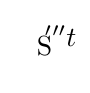
\begin{tikzpicture}[baseline=(top.base)]
                    \Tree [.\node(top){S}; [.DP [.D a ] [.NP [.N person ] ] ] [.XP [.1 ] [.S$'$ [.Neg not ] [.S$''$ [.NP [.N Bill ] ] [.VP [.V invite ] [.$t$ ] ] ] ] ] ]
                \end{tikzpicture}
            \ex \begin{tikzpicture}[baseline=(top.base)]
                    \Tree [.\node(top){S\,^{{\color{darkgray}\mathtt{FA\shortrightarrow}}}_{{\color{gray}t}} }; [.DP\,^{{\color{darkgray}\mathtt{FA\shortrightarrow}}}_{{\color{gray}\langle \langle e,\, t\rangle,\, t\rangle}} [.D\,^{{\color{darkgray}\mathtt{NN}}}_{{\color{gray}\langle \langle e,\, t\rangle,\, \langle \langle e,\, t\rangle,\, t\rangle\rangle}} a\,^{{\color{darkgray}\mathtt{TN_1}}}_{{\color{gray}\langle \langle e,\, t\rangle,\, \langle \langle e,\, t\rangle,\, t\rangle\rangle}} ] [.NP\,^{{\color{darkgray}\mathtt{NN}}}_{{\color{gray}\langle e,\, t\rangle}} [.N\,^{{\color{darkgray}\mathtt{NN}}}_{{\color{gray}\langle e,\, t\rangle}} person\,^{{\color{darkgray}\mathtt{TN_1}}}_{{\color{gray}\langle e,\, t\rangle}} ] ] ] [.XP\,^{{\color{darkgray}\mathtt{PA}}}_{{\color{gray}\langle e,\, t\rangle}} [.1\,^{{\color{darkgray}\mathtt{-}}}_{{\color{gray}-}} ] [.S$'$\,^{{\color{darkgray}\mathtt{FA\shortrightarrow}}}_{{\color{gray}t}} [.Neg\,^{{\color{darkgray}\mathtt{NN}}}_{{\color{gray}\langle t,\, t\rangle}} not\,^{{\color{darkgray}\mathtt{TN_1}}}_{{\color{gray}\langle t,\, t\rangle}} ] [.S$''$\,^{{\color{darkgray}\mathtt{FA\shortleftarrow}}}_{{\color{gray}t}} [.NP\,^{{\color{darkgray}\mathtt{NN}}}_{{\color{gray}e}} [.N\,^{{\color{darkgray}\mathtt{NN}}}_{{\color{gray}e}} Bill\,^{{\color{darkgray}\mathtt{TN_1}}}_{{\color{gray}e}} ] ] [.VP\,^{{\color{darkgray}\mathtt{FA\shortrightarrow}}}_{{\color{gray}\langle e,\, t\rangle}} [.V\,^{{\color{darkgray}\mathtt{NN}}}_{{\color{gray}\langle e,\, \langle e,\, t\rangle\rangle}} invite\,^{{\color{darkgray}\mathtt{TN_1}}}_{{\color{gray}\langle e,\, \langle e,\, t\rangle\rangle}} ] [.$t$\,^{{\color{darkgray}\mathtt{TN_2}}}_{{\color{gray}e}} ] ] ] ] ] ]
                \end{tikzpicture}
        \end{xlist}
    \end{exe}

\begin{exe}
    \ex Schuldiger Idiot.\hfill\textit{\footnotesize $2/15$ iterations, 0.57ms}
        \begin{xlist}
            % input string: "[.\node(top){NP}; [.AP schuldiger ] [.NP Idiot ] ]"
            \ex 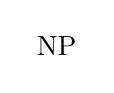
\begin{tikzpicture}[baseline=(top.base)]
                    \Tree [.\node(top){NP}; [.AP schuldiger ] [.NP Idiot ] ]
                \end{tikzpicture}
            \ex \begin{tikzpicture}[baseline=(top.base)]
                    \Tree [.\node(top){NP\,^{{\color{darkgray}\mathtt{PM}}}_{{\color{gray}\langle e,\, t\rangle}} }; [.AP\,^{{\color{darkgray}\mathtt{NN}}}_{{\color{gray}\langle e,\, t\rangle}} schuldiger\,^{{\color{darkgray}\mathtt{TN_1}}}_{{\color{gray}\langle e,\, t\rangle}} ] [.NP\,^{{\color{darkgray}\mathtt{NN}}}_{{\color{gray}\langle e,\, t\rangle}} Idiot\,^{{\color{darkgray}\mathtt{TN_1}}}_{{\color{gray}\langle e,\, t\rangle}} ] ]
                \end{tikzpicture}
        \end{xlist}
    \end{exe}

\begin{exe}
    \ex Some person is sad or she sleeps.\hfill\textit{\footnotesize $5/15$ iterations, 3.43ms}
        \begin{xlist}
            % input string: "[.\node(top){S}; [.S'' [.NP^1 [.Q some ] [.N^1 person ] ] [.VP [.V is ] [.AP [.A sad ] ] ] ] [.DisjP [.Disj or ] [.S' [.NP^2 [.N^2 she ] ] [.VP^2 [.V^2 sleeps ] ] ] ] ]"
            \ex \begin{tikzpicture}[baseline=(top.base)]
                    \Tree [.\node(top){S}; [.S'' [.NP [.Q some ] [.N person ] ] [.VP [.V is ] [.AP [.A sad ] ] ] ] [.DisjP [.Disj or ] [.S' [.NP [.N she ] ] [.VP [.V sleeps ] ] ] ] ]
                \end{tikzpicture}
            \ex \begin{tikzpicture}[baseline=(top.base)]
                    \Tree [.\node(top){S\,^{{\color{darkgray}\mathtt{FA\shortleftarrow}}}_{{\color{gray}t}} }; [.S''\,^{{\color{darkgray}\mathtt{FA\shortrightarrow}}}_{{\color{gray}t}} [.NP\,^{{\color{darkgray}\mathtt{FA\shortrightarrow}}}_{{\color{gray}\langle \langle e,\, t\rangle,\, t\rangle}} [.Q\,^{{\color{darkgray}\mathtt{NN}}}_{{\color{gray}\langle \langle e,\, t\rangle,\, \langle \langle e,\, t\rangle,\, t\rangle\rangle}} some\,^{{\color{darkgray}\mathtt{TN_1}}}_{{\color{gray}\langle \langle e,\, t\rangle,\, \langle \langle e,\, t\rangle,\, t\rangle\rangle}} ] [.N\,^{{\color{darkgray}\mathtt{NN}}}_{{\color{gray}\langle e,\, t\rangle}} person\,^{{\color{darkgray}\mathtt{TN_1}}}_{{\color{gray}\langle e,\, t\rangle}} ] ] [.VP\,^{{\color{darkgray}\mathtt{NN}}}_{{\color{gray}\langle e,\, t\rangle}} [.V\,^{{\color{darkgray}\mathtt{NN}}}_{{\color{gray}-}} is\,^{{\color{darkgray}\mathtt{-}}}_{{\color{gray}-}} ] [.AP\,^{{\color{darkgray}\mathtt{NN}}}_{{\color{gray}\langle e,\, t\rangle}} [.A\,^{{\color{darkgray}\mathtt{NN}}}_{{\color{gray}\langle e,\, t\rangle}} sad\,^{{\color{darkgray}\mathtt{TN_1}}}_{{\color{gray}\langle e,\, t\rangle}} ] ] ] ] [.DisjP\,^{{\color{darkgray}\mathtt{FA\shortrightarrow}}}_{{\color{gray}\langle t,\, t\rangle}} [.Disj\,^{{\color{darkgray}\mathtt{NN}}}_{{\color{gray}\langle t,\, \langle t,\, t\rangle\rangle}} or\,^{{\color{darkgray}\mathtt{TN_1}}}_{{\color{gray}\langle t,\, \langle t,\, t\rangle\rangle}} ] [.S'\,^{{\color{darkgray}\mathtt{FA\shortleftarrow}}}_{{\color{gray}t}} [.NP\,^{{\color{darkgray}\mathtt{NN}}}_{{\color{gray}e}} [.N\,^{{\color{darkgray}\mathtt{NN}}}_{{\color{gray}e}} she\,^{{\color{darkgray}\mathtt{TN_2}}}_{{\color{gray}e}} ] ] [.VP\,^{{\color{darkgray}\mathtt{NN}}}_{{\color{gray}\langle e,\, t\rangle}} [.V\,^{{\color{darkgray}\mathtt{NN}}}_{{\color{gray}\langle e,\, t\rangle}} sleeps\,^{{\color{darkgray}\mathtt{TN_1}}}_{{\color{gray}\langle e,\, t\rangle}} ] ] ] ] ]
                \end{tikzpicture}
        \end{xlist}
    \end{exe}

\begin{exe}
    \ex Alle Blumen beobachtet Peter.\hfill\textit{\footnotesize $4/15$ iterations, 0.84ms}
        \begin{xlist}
            % input string: "[.\node(top){S'}; [.NP^1 [.Q alle ] [.N^1 Blumen ] ] [.XP [.1 ] [.S [.VP [.V beobachtet ] [.$t$ ] ] [.NP^2 [.N^2 Peter ] ] ] ] ]"
            \ex 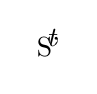
\begin{tikzpicture}[baseline=(top.base)]
                    \Tree [.\node(top){S'}; [.NP [.Q alle ] [.N Blumen ] ] [.XP [.1 ] [.S [.VP [.V beobachtet ] [.$t$ ] ] [.NP [.N Peter ] ] ] ] ]
                \end{tikzpicture}
            \ex \begin{tikzpicture}[baseline=(top.base)]
                    \Tree [.\node(top){S'\,^{{\color{darkgray}\mathtt{FA\shortrightarrow}}}_{{\color{gray}t}} }; [.NP\,^{{\color{darkgray}\mathtt{FA\shortrightarrow}}}_{{\color{gray}\langle \langle e,\, t\rangle,\, t\rangle}} [.Q\,^{{\color{darkgray}\mathtt{NN}}}_{{\color{gray}\langle \langle e,\, t\rangle,\, \langle \langle e,\, t\rangle,\, t\rangle\rangle}} alle\,^{{\color{darkgray}\mathtt{TN_1}}}_{{\color{gray}\langle \langle e,\, t\rangle,\, \langle \langle e,\, t\rangle,\, t\rangle\rangle}} ] [.N\,^{{\color{darkgray}\mathtt{NN}}}_{{\color{gray}\langle e,\, t\rangle}} Blumen\,^{{\color{darkgray}\mathtt{TN_1}}}_{{\color{gray}\langle e,\, t\rangle}} ] ] [.XP\,^{{\color{darkgray}\mathtt{PA}}}_{{\color{gray}\langle e,\, t\rangle}} [.1\,^{{\color{darkgray}\mathtt{-}}}_{{\color{gray}-}} ] [.S\,^{{\color{darkgray}\mathtt{FA\shortrightarrow}}}_{{\color{gray}t}} [.VP\,^{{\color{darkgray}\mathtt{FA\shortrightarrow}}}_{{\color{gray}\langle e,\, t\rangle}} [.V\,^{{\color{darkgray}\mathtt{NN}}}_{{\color{gray}\langle e,\, \langle e,\, t\rangle\rangle}} beobachtet\,^{{\color{darkgray}\mathtt{TN_1}}}_{{\color{gray}\langle e,\, \langle e,\, t\rangle\rangle}} ] [.$t$\,^{{\color{darkgray}\mathtt{TN_2}}}_{{\color{gray}e}} ] ] [.NP\,^{{\color{darkgray}\mathtt{NN}}}_{{\color{gray}e}} [.N\,^{{\color{darkgray}\mathtt{NN}}}_{{\color{gray}e}} Peter\,^{{\color{darkgray}\mathtt{TN_1}}}_{{\color{gray}e}} ] ] ] ] ]
                \end{tikzpicture}
        \end{xlist}
    \end{exe}

\begin{exe}
    \ex Peter ist ein fliegender Junge aus Nimmerland.\hfill\textit{\footnotesize $6/15$ iterations, 1.93ms}
        \begin{xlist}
            % input string: "[.\node(top){S}; [.NP^1 [.N^1 Peter ] ] [.VP [.V ist ] [.DP [.D ein ] [.NP^2 [.N$''$^2 [.AP [.A fliegender ] ] [.N$'$^2 [.N^2 Junge ] ] ] [.PP [.P aus ] [.NP^3 [.N^3 Nimmerland ] ] ] ] ] ] ]"
            \ex 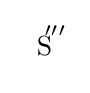
\begin{tikzpicture}[baseline=(top.base)]
                    \Tree [.\node(top){S}; [.NP [.N Peter ] ] [.VP [.V ist ] [.DP [.D ein ] [.NP [.N$''$ [.AP [.A fliegender ] ] [.N$'$ [.N Junge ] ] ] [.PP [.P aus ] [.NP [.N Nimmerland ] ] ] ] ] ] ]
                \end{tikzpicture}
            \ex \begin{tikzpicture}[baseline=(top.base)]
                    \Tree [.\node(top){S\,^{{\color{darkgray}\mathtt{FA\shortleftarrow}}}_{{\color{gray}t}} }; [.NP\,^{{\color{darkgray}\mathtt{NN}}}_{{\color{gray}e}} [.N\,^{{\color{darkgray}\mathtt{NN}}}_{{\color{gray}e}} Peter\,^{{\color{darkgray}\mathtt{TN_1}}}_{{\color{gray}e}} ] ] [.VP\,^{{\color{darkgray}\mathtt{NN}}}_{{\color{gray}\langle e,\, t\rangle}} [.V\,^{{\color{darkgray}\mathtt{NN}}}_{{\color{gray}-}} ist\,^{{\color{darkgray}\mathtt{-}}}_{{\color{gray}-}} ] [.DP\,^{{\color{darkgray}\mathtt{NN}}}_{{\color{gray}\langle e,\, t\rangle}} [.D\,^{{\color{darkgray}\mathtt{NN}}}_{{\color{gray}-}} ein\,^{{\color{darkgray}\mathtt{-}}}_{{\color{gray}-}} ] [.NP\,^{{\color{darkgray}\mathtt{PM}}}_{{\color{gray}\langle e,\, t\rangle}} [.N$''$\,^{{\color{darkgray}\mathtt{PM}}}_{{\color{gray}\langle e,\, t\rangle}} [.AP\,^{{\color{darkgray}\mathtt{NN}}}_{{\color{gray}\langle e,\, t\rangle}} [.A\,^{{\color{darkgray}\mathtt{NN}}}_{{\color{gray}\langle e,\, t\rangle}} fliegender\,^{{\color{darkgray}\mathtt{TN_1}}}_{{\color{gray}\langle e,\, t\rangle}} ] ] [.N$'$\,^{{\color{darkgray}\mathtt{NN}}}_{{\color{gray}\langle e,\, t\rangle}} [.N\,^{{\color{darkgray}\mathtt{NN}}}_{{\color{gray}\langle e,\, t\rangle}} Junge\,^{{\color{darkgray}\mathtt{TN_1}}}_{{\color{gray}\langle e,\, t\rangle}} ] ] ] [.PP\,^{{\color{darkgray}\mathtt{FA\shortrightarrow}}}_{{\color{gray}\langle e,\, t\rangle}} [.P\,^{{\color{darkgray}\mathtt{NN}}}_{{\color{gray}\langle e,\, \langle e,\, t\rangle\rangle}} aus\,^{{\color{darkgray}\mathtt{TN_1}}}_{{\color{gray}\langle e,\, \langle e,\, t\rangle\rangle}} ] [.NP\,^{{\color{darkgray}\mathtt{NN}}}_{{\color{gray}e}} [.N\,^{{\color{darkgray}\mathtt{NN}}}_{{\color{gray}e}} Nimmerland\,^{{\color{darkgray}\mathtt{TN_1}}}_{{\color{gray}e}} ] ] ] ] ] ] ]
                \end{tikzpicture}
        \end{xlist}
    \end{exe}

\begin{exe}
    \ex Er ist stolz auf Maria.\hfill\textit{\footnotesize $5/15$ iterations, 1.12ms}
        \begin{xlist}
            % input string: "[.\node(top){S}; [.NP [.N er ] ] [.VP [.V ist ] [.AP [.A stolz ] [.PP [.P auf ] [.NP^2 [.N^2 Maria ] ] ] ] ] ]"
            \ex \begin{tikzpicture}[baseline=(top.base)]
                    \Tree [.\node(top){S}; [.NP [.N er ] ] [.VP [.V ist ] [.AP [.A stolz ] [.PP [.P auf ] [.NP [.N Maria ] ] ] ] ] ]
                \end{tikzpicture}
            \ex \begin{tikzpicture}[baseline=(top.base)]
                    \Tree [.\node(top){S\,^{{\color{darkgray}\mathtt{FA\shortleftarrow}}}_{{\color{gray}t}} }; [.NP\,^{{\color{darkgray}\mathtt{NN}}}_{{\color{gray}e}} [.N\,^{{\color{darkgray}\mathtt{NN}}}_{{\color{gray}e}} er\,^{{\color{darkgray}\mathtt{TN_2}}}_{{\color{gray}e}} ] ] [.VP\,^{{\color{darkgray}\mathtt{NN}}}_{{\color{gray}\langle e,\, t\rangle}} [.V\,^{{\color{darkgray}\mathtt{NN}}}_{{\color{gray}-}} ist\,^{{\color{darkgray}\mathtt{-}}}_{{\color{gray}-}} ] [.AP\,^{{\color{darkgray}\mathtt{FA\shortrightarrow}}}_{{\color{gray}\langle e,\, t\rangle}} [.A\,^{{\color{darkgray}\mathtt{NN}}}_{{\color{gray}\langle e,\, \langle e,\, t\rangle\rangle}} stolz\,^{{\color{darkgray}\mathtt{TN_1}}}_{{\color{gray}\langle e,\, \langle e,\, t\rangle\rangle}} ] [.PP\,^{{\color{darkgray}\mathtt{NN}}}_{{\color{gray}e}} [.P\,^{{\color{darkgray}\mathtt{NN}}}_{{\color{gray}-}} auf\,^{{\color{darkgray}\mathtt{-}}}_{{\color{gray}-}} ] [.NP\,^{{\color{darkgray}\mathtt{NN}}}_{{\color{gray}e}} [.N\,^{{\color{darkgray}\mathtt{NN}}}_{{\color{gray}e}} Maria\,^{{\color{darkgray}\mathtt{TN_1}}}_{{\color{gray}e}} ] ] ] ] ] ]
                \end{tikzpicture}
        \end{xlist}
    \end{exe}

\begin{exe}
    \ex Einige schnarchende Jungen zwicken die kleinen Männer.\hfill\textit{\footnotesize $6/15$ iterations, 2.11ms}
        \begin{xlist}
            % input string: "[.\node(top){S}; [.NP [.Q einige ] [.N' [.AP^1 [.A^1 schnarchende ] ] [.N'' [.N Jungen ] ] ] ] [.VP [.V zwicken ] [.NP^2 [.D die ] [.N'^2 [.AP^2 [.A^2 kleinen ] ] [.N^2 Männer ] ] ] ] ]"
            \ex \begin{tikzpicture}[baseline=(top.base)]
                    \Tree [.\node(top){S}; [.NP [.Q einige ] [.N' [.AP [.A schnarchende ] ] [.N'' [.N Jungen ] ] ] ] [.VP [.V zwicken ] [.NP [.D die ] [.N' [.AP [.A kleinen ] ] [.N Männer ] ] ] ] ]
                \end{tikzpicture}
            \ex \begin{tikzpicture}[baseline=(top.base)]
                    \Tree [.\node(top){S\,^{{\color{darkgray}\mathtt{FA\shortrightarrow}}}_{{\color{gray}t}} }; [.NP\,^{{\color{darkgray}\mathtt{FA\shortrightarrow}}}_{{\color{gray}\langle \langle e,\, t\rangle,\, t\rangle}} [.Q\,^{{\color{darkgray}\mathtt{NN}}}_{{\color{gray}\langle \langle e,\, t\rangle,\, \langle \langle e,\, t\rangle,\, t\rangle\rangle}} einige\,^{{\color{darkgray}\mathtt{TN_1}}}_{{\color{gray}\langle \langle e,\, t\rangle,\, \langle \langle e,\, t\rangle,\, t\rangle\rangle}} ] [.N'\,^{{\color{darkgray}\mathtt{PM}}}_{{\color{gray}\langle e,\, t\rangle}} [.AP\,^{{\color{darkgray}\mathtt{NN}}}_{{\color{gray}\langle e,\, t\rangle}} [.A\,^{{\color{darkgray}\mathtt{NN}}}_{{\color{gray}\langle e,\, t\rangle}} schnarchende\,^{{\color{darkgray}\mathtt{TN_1}}}_{{\color{gray}\langle e,\, t\rangle}} ] ] [.N''\,^{{\color{darkgray}\mathtt{NN}}}_{{\color{gray}\langle e,\, t\rangle}} [.N\,^{{\color{darkgray}\mathtt{NN}}}_{{\color{gray}\langle e,\, t\rangle}} Jungen\,^{{\color{darkgray}\mathtt{TN_1}}}_{{\color{gray}\langle e,\, t\rangle}} ] ] ] ] [.VP\,^{{\color{darkgray}\mathtt{FA\shortrightarrow}}}_{{\color{gray}\langle e,\, t\rangle}} [.V\,^{{\color{darkgray}\mathtt{NN}}}_{{\color{gray}\langle e,\, \langle e,\, t\rangle\rangle}} zwicken\,^{{\color{darkgray}\mathtt{TN_1}}}_{{\color{gray}\langle e,\, \langle e,\, t\rangle\rangle}} ] [.NP\,^{{\color{darkgray}\mathtt{FA\shortrightarrow}}}_{{\color{gray}e}} [.D\,^{{\color{darkgray}\mathtt{NN}}}_{{\color{gray}\langle \langle e,\, t\rangle,\, e\rangle}} die\,^{{\color{darkgray}\mathtt{TN_1}}}_{{\color{gray}\langle \langle e,\, t\rangle,\, e\rangle}} ] [.N'\,^{{\color{darkgray}\mathtt{PM}}}_{{\color{gray}\langle e,\, t\rangle}} [.AP\,^{{\color{darkgray}\mathtt{NN}}}_{{\color{gray}\langle e,\, t\rangle}} [.A\,^{{\color{darkgray}\mathtt{NN}}}_{{\color{gray}\langle e,\, t\rangle}} kleinen\,^{{\color{darkgray}\mathtt{TN_1}}}_{{\color{gray}\langle e,\, t\rangle}} ] ] [.N\,^{{\color{darkgray}\mathtt{NN}}}_{{\color{gray}\langle e,\, t\rangle}} Männer\,^{{\color{darkgray}\mathtt{TN_1}}}_{{\color{gray}\langle e,\, t\rangle}} ] ] ] ] ]
                \end{tikzpicture}
        \end{xlist}
    \end{exe}

\begin{exe}
    \ex Der Junge der_{RP} wo die Fee aus Nimmerland belästigt fliegt.\hfill\textit{\footnotesize $9/15$ iterations, 3.95ms}
        \begin{xlist}
            % input string: "[.\node(top){S}; [.DP^1 [.D^1 der ] [.NP [.N$''$ [.N$'$ [.N Junge ] ] [.CP [.DP^2 der_{RP}_1 ] [.C$'$ [.C wo ] [.S$'$ [.$t$_1 ] [.VP [.DP^3 [.D^3 die ] [.NP^2 [.N$''$^2 [.N$'$^2 [.N^2 Fee ] ] [.PP [.P aus ] [.DP^4 Nimmerland ] ] ] ] ]  [.V belästigt ] ] ] ] ] ] ] ]  [.VP^2 [.V^2 fliegt ] ] ]"
            \ex \begin{tikzpicture}[baseline=(top.base)]
                    \Tree [.\node(top){S}; [.DP [.D der ] [.NP [.N$''$ [.N$'$ [.N Junge ] ] [.CP [.DP der_{RP}_1 ] [.C$'$ [.C wo ] [.S$'$ [.$t$_1 ] [.VP [.DP [.D die ] [.NP [.N$''$ [.N$'$ [.N Fee ] ] [.PP [.P aus ] [.DP Nimmerland ] ] ] ] ]  [.V belästigt ] ] ] ] ] ] ] ]  [.VP [.V fliegt ] ] ]
                \end{tikzpicture}
            \ex \begin{tikzpicture}[baseline=(top.base)]
                    \Tree [.\node(top){S\,^{{\color{darkgray}\mathtt{FA\shortleftarrow}}}_{{\color{gray}t}} }; [.DP\,^{{\color{darkgray}\mathtt{FA\shortrightarrow}}}_{{\color{gray}e}} [.D\,^{{\color{darkgray}\mathtt{NN}}}_{{\color{gray}\langle \langle e,\, t\rangle,\, e\rangle}} der\,^{{\color{darkgray}\mathtt{TN_1}}}_{{\color{gray}\langle \langle e,\, t\rangle,\, e\rangle}} ] [.NP\,^{{\color{darkgray}\mathtt{NN}}}_{{\color{gray}\langle e,\, t\rangle}} [.N$''$\,^{{\color{darkgray}\mathtt{PM}}}_{{\color{gray}\langle e,\, t\rangle}} [.N$'$\,^{{\color{darkgray}\mathtt{NN}}}_{{\color{gray}\langle e,\, t\rangle}} [.N\,^{{\color{darkgray}\mathtt{NN}}}_{{\color{gray}\langle e,\, t\rangle}} Junge\,^{{\color{darkgray}\mathtt{TN_1}}}_{{\color{gray}\langle e,\, t\rangle}} ] ] [.CP\,^{{\color{darkgray}\mathtt{PA}}}_{{\color{gray}\langle e,\, t\rangle}} [.DP\,^{{\color{darkgray}\mathtt{NN}}}_{{\color{gray}-}} der_{RP}\,^{{\color{darkgray}\mathtt{-}}}_{{\color{gray}-}} ] [.C$'$\,^{{\color{darkgray}\mathtt{NN}}}_{{\color{gray}t}} [.C\,^{{\color{darkgray}\mathtt{NN}}}_{{\color{gray}-}} wo\,^{{\color{darkgray}\mathtt{-}}}_{{\color{gray}-}} ] [.S$'$\,^{{\color{darkgray}\mathtt{FA\shortleftarrow}}}_{{\color{gray}t}} [.$t$\,^{{\color{darkgray}\mathtt{TN_2}}}_{{\color{gray}e}} ] [.VP\,^{{\color{darkgray}\mathtt{FA\shortleftarrow}}}_{{\color{gray}\langle e,\, t\rangle}} [.DP\,^{{\color{darkgray}\mathtt{FA\shortrightarrow}}}_{{\color{gray}e}} [.D\,^{{\color{darkgray}\mathtt{NN}}}_{{\color{gray}\langle \langle e,\, t\rangle,\, e\rangle}} die\,^{{\color{darkgray}\mathtt{TN_1}}}_{{\color{gray}\langle \langle e,\, t\rangle,\, e\rangle}} ] [.NP\,^{{\color{darkgray}\mathtt{NN}}}_{{\color{gray}\langle e,\, t\rangle}} [.N$''$\,^{{\color{darkgray}\mathtt{PM}}}_{{\color{gray}\langle e,\, t\rangle}} [.N$'$\,^{{\color{darkgray}\mathtt{NN}}}_{{\color{gray}\langle e,\, t\rangle}} [.N\,^{{\color{darkgray}\mathtt{NN}}}_{{\color{gray}\langle e,\, t\rangle}} Fee\,^{{\color{darkgray}\mathtt{TN_1}}}_{{\color{gray}\langle e,\, t\rangle}} ] ] [.PP\,^{{\color{darkgray}\mathtt{FA\shortrightarrow}}}_{{\color{gray}\langle e,\, t\rangle}} [.P\,^{{\color{darkgray}\mathtt{NN}}}_{{\color{gray}\langle e,\, \langle e,\, t\rangle\rangle}} aus\,^{{\color{darkgray}\mathtt{TN_1}}}_{{\color{gray}\langle e,\, \langle e,\, t\rangle\rangle}} ] [.DP\,^{{\color{darkgray}\mathtt{NN}}}_{{\color{gray}e}} Nimmerland\,^{{\color{darkgray}\mathtt{TN_1}}}_{{\color{gray}e}} ] ] ] ] ]  [.V\,^{{\color{darkgray}\mathtt{NN}}}_{{\color{gray}\langle e,\, \langle e,\, t\rangle\rangle}} belästigt\,^{{\color{darkgray}\mathtt{TN_1}}}_{{\color{gray}\langle e,\, \langle e,\, t\rangle\rangle}} ] ] ] ] ] ] ] ]  [.VP\,^{{\color{darkgray}\mathtt{NN}}}_{{\color{gray}\langle e,\, t\rangle}} [.V\,^{{\color{darkgray}\mathtt{NN}}}_{{\color{gray}\langle e,\, t\rangle}} fliegt\,^{{\color{darkgray}\mathtt{TN_1}}}_{{\color{gray}\langle e,\, t\rangle}} ] ] ]
                \end{tikzpicture}
        \end{xlist}
    \end{exe}

\begin{exe}
    \ex Der Junge der_{RP} wo die Fee aus Nimmerland belästigt fliegt.\hfill\textit{\footnotesize $9/15$ iterations, 1.41ms}
        \begin{xlist}
            % input string: "[.S [.DP^1 [.D^1 der ] [.NP [.N$''$ [.N$'$ [.N Junge ] ] [.CP [.DP^2 der_{RP} ] [.C$'$ [.C wo ] [.S$'$ [.$t$_{1} ] [.VP [.DP^3 [.D^3 die ] [.NP^2 [.N$''$^2 [.N$'$^2 [.N^2 Fee ] ] [.PP [.P aus ] [.DP^4 Nimmerland ] ] ] ] ]  [.V belästigt ] ] ] ] ] ] ] ]  [.VP^2 [.V^2 fliegt ] ] ]"
            \ex \begin{tikzpicture}[baseline=(top.base)]
                    \Tree [.\node(top){S}; [.DP [.D der ] [.NP [.N$''$ [.N$'$ [.N Junge ] ] [.CP [.DP der_{RP} ] [.C$'$ [.C wo ] [.S$'$ [.$t$_{1} ] [.VP [.DP [.D die ] [.NP [.N$''$ [.N$'$ [.N Fee ] ] [.PP [.P aus ] [.DP Nimmerland ] ] ] ] ]  [.V belästigt ] ] ] ] ] ] ] ]  [.VP [.V fliegt ] ] ]
                \end{tikzpicture}
            \ex \begin{tikzpicture}[baseline=(top.base)]
                    \Tree [.\node(top){S\,^{{\color{darkgray}\mathtt{FA\shortleftarrow}}}_{{\color{gray}t}} }; [.DP\,^{{\color{darkgray}\mathtt{FA\shortrightarrow}}}_{{\color{gray}e}} [.D\,^{{\color{darkgray}\mathtt{NN}}}_{{\color{gray}\langle \langle e,\, t\rangle,\, e\rangle}} der\,^{{\color{darkgray}\mathtt{TN_1}}}_{{\color{gray}\langle \langle e,\, t\rangle,\, e\rangle}} ] [.NP\,^{{\color{darkgray}\mathtt{NN}}}_{{\color{gray}\langle e,\, t\rangle}} [.N$''$\,^{{\color{darkgray}\mathtt{PM}}}_{{\color{gray}\langle e,\, t\rangle}} [.N$'$\,^{{\color{darkgray}\mathtt{NN}}}_{{\color{gray}\langle e,\, t\rangle}} [.N\,^{{\color{darkgray}\mathtt{NN}}}_{{\color{gray}\langle e,\, t\rangle}} Junge\,^{{\color{darkgray}\mathtt{TN_1}}}_{{\color{gray}\langle e,\, t\rangle}} ] ] [.CP\,^{{\color{darkgray}\mathtt{PA}}}_{{\color{gray}\langle e,\, t\rangle}} [.DP\,^{{\color{darkgray}\mathtt{NN}}}_{{\color{gray}-}} der_{RP}\,^{{\color{darkgray}\mathtt{-}}}_{{\color{gray}-}} ] [.C$'$\,^{{\color{darkgray}\mathtt{NN}}}_{{\color{gray}t}} [.C\,^{{\color{darkgray}\mathtt{NN}}}_{{\color{gray}-}} wo\,^{{\color{darkgray}\mathtt{-}}}_{{\color{gray}-}} ] [.S$'$\,^{{\color{darkgray}\mathtt{FA\shortleftarrow}}}_{{\color{gray}t}} [.$t$\,^{{\color{darkgray}\mathtt{TN_2}}}_{{\color{gray}e}} ] [.VP\,^{{\color{darkgray}\mathtt{FA\shortleftarrow}}}_{{\color{gray}\langle e,\, t\rangle}} [.DP\,^{{\color{darkgray}\mathtt{FA\shortrightarrow}}}_{{\color{gray}e}} [.D\,^{{\color{darkgray}\mathtt{NN}}}_{{\color{gray}\langle \langle e,\, t\rangle,\, e\rangle}} die\,^{{\color{darkgray}\mathtt{TN_1}}}_{{\color{gray}\langle \langle e,\, t\rangle,\, e\rangle}} ] [.NP\,^{{\color{darkgray}\mathtt{NN}}}_{{\color{gray}\langle e,\, t\rangle}} [.N$''$\,^{{\color{darkgray}\mathtt{PM}}}_{{\color{gray}\langle e,\, t\rangle}} [.N$'$\,^{{\color{darkgray}\mathtt{NN}}}_{{\color{gray}\langle e,\, t\rangle}} [.N\,^{{\color{darkgray}\mathtt{NN}}}_{{\color{gray}\langle e,\, t\rangle}} Fee\,^{{\color{darkgray}\mathtt{TN_1}}}_{{\color{gray}\langle e,\, t\rangle}} ] ] [.PP\,^{{\color{darkgray}\mathtt{FA\shortrightarrow}}}_{{\color{gray}\langle e,\, t\rangle}} [.P\,^{{\color{darkgray}\mathtt{NN}}}_{{\color{gray}\langle e,\, \langle e,\, t\rangle\rangle}} aus\,^{{\color{darkgray}\mathtt{TN_1}}}_{{\color{gray}\langle e,\, \langle e,\, t\rangle\rangle}} ] [.DP\,^{{\color{darkgray}\mathtt{NN}}}_{{\color{gray}e}} Nimmerland\,^{{\color{darkgray}\mathtt{TN_1}}}_{{\color{gray}e}} ] ] ] ] ]  [.V\,^{{\color{darkgray}\mathtt{NN}}}_{{\color{gray}\langle e,\, \langle e,\, t\rangle\rangle}} belästigt\,^{{\color{darkgray}\mathtt{TN_1}}}_{{\color{gray}\langle e,\, \langle e,\, t\rangle\rangle}} ] ] ] ] ] ] ] ]  [.VP\,^{{\color{darkgray}\mathtt{NN}}}_{{\color{gray}\langle e,\, t\rangle}} [.V\,^{{\color{darkgray}\mathtt{NN}}}_{{\color{gray}\langle e,\, t\rangle}} fliegt\,^{{\color{darkgray}\mathtt{TN_1}}}_{{\color{gray}\langle e,\, t\rangle}} ] ] ]
                \end{tikzpicture}
        \end{xlist}
    \end{exe}

\begin{exe}
    \ex Dem Schüler das Buch Bill gibt.\hfill\textit{\footnotesize $6/15$ iterations, 2.35ms}
        \begin{xlist}
            % input string: "[.\node(top){WP}; [.DP^2 [.D^2 dem ] [.NP^2 [.N^2 Schüler ] ] ] [.ZP [.2 ] [.XP [.DP^1 [.D^1 das ] [.NP^1 [.N^1 Buch ] ] ] [.YP [.1 ] [.S [.NP^3 [.N^3 Bill ] ] [.VP [.V$'$ [.V gibt ] [.$t$ ] ] [.$t$ ] ] ] ] ] ] ]"
            \ex 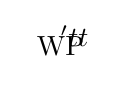
\begin{tikzpicture}[baseline=(top.base)]
                    \Tree [.\node(top){WP}; [.DP [.D dem ] [.NP [.N Schüler ] ] ] [.ZP [.2 ] [.XP [.DP [.D das ] [.NP [.N Buch ] ] ] [.YP [.1 ] [.S [.NP [.N Bill ] ] [.VP [.V$'$ [.V gibt ] [.$t$ ] ] [.$t$ ] ] ] ] ] ] ]
                \end{tikzpicture}
            \ex \begin{tikzpicture}[baseline=(top.base)]
                    \Tree [.\node(top){WP\,^{{\color{darkgray}\mathtt{FA\shortleftarrow}}}_{{\color{gray}t}} }; [.DP\,^{{\color{darkgray}\mathtt{FA\shortrightarrow}}}_{{\color{gray}e}} [.D\,^{{\color{darkgray}\mathtt{NN}}}_{{\color{gray}\langle \langle e,\, t\rangle,\, e\rangle}} dem\,^{{\color{darkgray}\mathtt{TN_1}}}_{{\color{gray}\langle \langle e,\, t\rangle,\, e\rangle}} ] [.NP\,^{{\color{darkgray}\mathtt{NN}}}_{{\color{gray}\langle e,\, t\rangle}} [.N\,^{{\color{darkgray}\mathtt{NN}}}_{{\color{gray}\langle e,\, t\rangle}} Schüler\,^{{\color{darkgray}\mathtt{TN_1}}}_{{\color{gray}\langle e,\, t\rangle}} ] ] ] [.ZP\,^{{\color{darkgray}\mathtt{PA}}}_{{\color{gray}\langle e,\, t\rangle}} [.2\,^{{\color{darkgray}\mathtt{-}}}_{{\color{gray}-}} ] [.XP\,^{{\color{darkgray}\mathtt{FA\shortleftarrow}}}_{{\color{gray}t}} [.DP\,^{{\color{darkgray}\mathtt{FA\shortrightarrow}}}_{{\color{gray}e}} [.D\,^{{\color{darkgray}\mathtt{NN}}}_{{\color{gray}\langle \langle e,\, t\rangle,\, e\rangle}} das\,^{{\color{darkgray}\mathtt{TN_1}}}_{{\color{gray}\langle \langle e,\, t\rangle,\, e\rangle}} ] [.NP\,^{{\color{darkgray}\mathtt{NN}}}_{{\color{gray}\langle e,\, t\rangle}} [.N\,^{{\color{darkgray}\mathtt{NN}}}_{{\color{gray}\langle e,\, t\rangle}} Buch\,^{{\color{darkgray}\mathtt{TN_1}}}_{{\color{gray}\langle e,\, t\rangle}} ] ] ] [.YP\,^{{\color{darkgray}\mathtt{PA}}}_{{\color{gray}\langle e,\, t\rangle}} [.1\,^{{\color{darkgray}\mathtt{-}}}_{{\color{gray}-}} ] [.S\,^{{\color{darkgray}\mathtt{FA\shortleftarrow}}}_{{\color{gray}t}} [.NP\,^{{\color{darkgray}\mathtt{NN}}}_{{\color{gray}e}} [.N\,^{{\color{darkgray}\mathtt{NN}}}_{{\color{gray}e}} Bill\,^{{\color{darkgray}\mathtt{TN_1}}}_{{\color{gray}e}} ] ] [.VP\,^{{\color{darkgray}\mathtt{FA\shortrightarrow}}}_{{\color{gray}\langle e,\, t\rangle}} [.V$'$\,^{{\color{darkgray}\mathtt{FA\shortrightarrow}}}_{{\color{gray}\langle e,\, \langle e,\, t\rangle\rangle}} [.V\,^{{\color{darkgray}\mathtt{NN}}}_{{\color{gray}\langle e,\, \langle e,\, \langle e,\, t\rangle\rangle\rangle}} gibt\,^{{\color{darkgray}\mathtt{TN_1}}}_{{\color{gray}\langle e,\, \langle e,\, \langle e,\, t\rangle\rangle\rangle}} ] [.$t$\,^{{\color{darkgray}\mathtt{TN_2}}}_{{\color{gray}e}} ] ] [.$t$\,^{{\color{darkgray}\mathtt{TN_2}}}_{{\color{gray}e}} ] ] ] ] ] ] ]
                \end{tikzpicture}
        \end{xlist}
    \end{exe}

\begin{exe}
    \ex Alle Hunde einige Türen schließen.\hfill\textit{\footnotesize $5/15$ iterations, 1.44ms}
        \begin{xlist}
            % input string: "[.\node(top){S$'$}; [.DP^2 [.D^2 alle ] [.NP^2 [.N^2 Hunde ] ] ] [.XP [.2 ] [.YP [.DP^1 [.D^1 einige ] [.NP^1 [.N^1 Türen ] ] ] [.ZP [.1 ] [.S [.$t$ ] [.VP [.V schließen ] [.$t$ ] ] ] ] ] ] ]"
            \ex 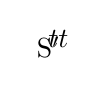
\begin{tikzpicture}[baseline=(top.base)]
                    \Tree [.\node(top){S$'$}; [.DP [.D alle ] [.NP [.N Hunde ] ] ] [.XP [.2 ] [.YP [.DP [.D einige ] [.NP [.N Türen ] ] ] [.ZP [.1 ] [.S [.$t$ ] [.VP [.V schließen ] [.$t$ ] ] ] ] ] ] ]
                \end{tikzpicture}
            \ex \begin{tikzpicture}[baseline=(top.base)]
                    \Tree [.\node(top){S$'$\,^{{\color{darkgray}\mathtt{FA\shortrightarrow}}}_{{\color{gray}t}} }; [.DP\,^{{\color{darkgray}\mathtt{FA\shortrightarrow}}}_{{\color{gray}\langle \langle e,\, t\rangle,\, t\rangle}} [.D\,^{{\color{darkgray}\mathtt{NN}}}_{{\color{gray}\langle \langle e,\, t\rangle,\, \langle \langle e,\, t\rangle,\, t\rangle\rangle}} alle\,^{{\color{darkgray}\mathtt{TN_1}}}_{{\color{gray}\langle \langle e,\, t\rangle,\, \langle \langle e,\, t\rangle,\, t\rangle\rangle}} ] [.NP\,^{{\color{darkgray}\mathtt{NN}}}_{{\color{gray}\langle e,\, t\rangle}} [.N\,^{{\color{darkgray}\mathtt{NN}}}_{{\color{gray}\langle e,\, t\rangle}} Hunde\,^{{\color{darkgray}\mathtt{TN_1}}}_{{\color{gray}\langle e,\, t\rangle}} ] ] ] [.XP\,^{{\color{darkgray}\mathtt{PA}}}_{{\color{gray}\langle e,\, t\rangle}} [.2\,^{{\color{darkgray}\mathtt{-}}}_{{\color{gray}-}} ] [.YP\,^{{\color{darkgray}\mathtt{FA\shortrightarrow}}}_{{\color{gray}t}} [.DP\,^{{\color{darkgray}\mathtt{FA\shortrightarrow}}}_{{\color{gray}\langle \langle e,\, t\rangle,\, t\rangle}} [.D\,^{{\color{darkgray}\mathtt{NN}}}_{{\color{gray}\langle \langle e,\, t\rangle,\, \langle \langle e,\, t\rangle,\, t\rangle\rangle}} einige\,^{{\color{darkgray}\mathtt{TN_1}}}_{{\color{gray}\langle \langle e,\, t\rangle,\, \langle \langle e,\, t\rangle,\, t\rangle\rangle}} ] [.NP\,^{{\color{darkgray}\mathtt{NN}}}_{{\color{gray}\langle e,\, t\rangle}} [.N\,^{{\color{darkgray}\mathtt{NN}}}_{{\color{gray}\langle e,\, t\rangle}} Türen\,^{{\color{darkgray}\mathtt{TN_1}}}_{{\color{gray}\langle e,\, t\rangle}} ] ] ] [.ZP\,^{{\color{darkgray}\mathtt{PA}}}_{{\color{gray}\langle e,\, t\rangle}} [.1\,^{{\color{darkgray}\mathtt{-}}}_{{\color{gray}-}} ] [.S\,^{{\color{darkgray}\mathtt{FA\shortleftarrow}}}_{{\color{gray}t}} [.$t$\,^{{\color{darkgray}\mathtt{TN_2}}}_{{\color{gray}e}} ] [.VP\,^{{\color{darkgray}\mathtt{FA\shortrightarrow}}}_{{\color{gray}\langle e,\, t\rangle}} [.V\,^{{\color{darkgray}\mathtt{NN}}}_{{\color{gray}\langle e,\, \langle e,\, t\rangle\rangle}} schließen\,^{{\color{darkgray}\mathtt{TN_1}}}_{{\color{gray}\langle e,\, \langle e,\, t\rangle\rangle}} ] [.$t$\,^{{\color{darkgray}\mathtt{TN_2}}}_{{\color{gray}e}} ] ] ] ] ] ] ]
                \end{tikzpicture}
        \end{xlist}
    \end{exe}

\begin{exe}
    \ex Maria -s snore.\hfill\textit{\footnotesize $5/15$ iterations, 1.31ms}
        \begin{xlist}
            % input string: "[.\node(top){TP}; [.DP Maria ] [.T'' [.1 ] [.T' [.T^0 -s ] [.VP [.t ] [.V$'$ [.V^0 snore ] ] ] ] ] ]"
            \ex 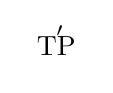
\begin{tikzpicture}[baseline=(top.base)]
                    \Tree [.\node(top){TP}; [.DP Maria ] [.T'' [.1 ] [.T' [.T -s ] [.VP [.t ] [.V$'$ [.V snore ] ] ] ] ] ]
                \end{tikzpicture}
            \ex \begin{tikzpicture}[baseline=(top.base)]
                    \Tree [.\node(top){TP\,^{{\color{darkgray}\mathtt{FA\shortleftarrow}}}_{{\color{gray}t}} }; [.DP\,^{{\color{darkgray}\mathtt{NN}}}_{{\color{gray}e}} Maria\,^{{\color{darkgray}\mathtt{TN_1}}}_{{\color{gray}e}} ] [.T''\,^{{\color{darkgray}\mathtt{PA}}}_{{\color{gray}\langle e,\, t\rangle}} [.1\,^{{\color{darkgray}\mathtt{-}}}_{{\color{gray}-}} ] [.T'\,^{{\color{darkgray}\mathtt{NN}}}_{{\color{gray}t}} [.T\,^{{\color{darkgray}\mathtt{NN}}}_{{\color{gray}-}} -s\,^{{\color{darkgray}\mathtt{-}}}_{{\color{gray}-}} ] [.VP\,^{{\color{darkgray}\mathtt{FA\shortleftarrow}}}_{{\color{gray}t}} [.t\,^{{\color{darkgray}\mathtt{TN_2}}}_{{\color{gray}e}} ] [.V$'$\,^{{\color{darkgray}\mathtt{NN}}}_{{\color{gray}\langle e,\, t\rangle}} [.V\,^{{\color{darkgray}\mathtt{NN}}}_{{\color{gray}\langle e,\, t\rangle}} snore\,^{{\color{darkgray}\mathtt{TN_1}}}_{{\color{gray}\langle e,\, t\rangle}} ] ] ] ] ] ]
                \end{tikzpicture}
        \end{xlist}
    \end{exe}

\begin{exe}
    \ex Das essen $t$.\hfill\textit{\footnotesize $2/15$ iterations, 0.52ms}
        \begin{xlist}
            % input string: "[.\node(top){S}; [.DP [.D^0 das ] [.NP essen ] ] [.VP $t$ ] ]"
            \ex 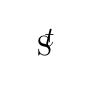
\begin{tikzpicture}[baseline=(top.base)]
                    \Tree [.\node(top){S}; [.DP [.D das ] [.NP essen ] ] [.VP $t$ ] ]
                \end{tikzpicture}
            \ex \begin{tikzpicture}[baseline=(top.base)]
                    \Tree [.\node(top){S\,^{{\color{red}\mathtt{?}}}_{{\color{red}?}} }; [.DP\,^{{\color{darkgray}\mathtt{FA\shortrightarrow}}}_{{\color{gray}e}} [.D\,^{{\color{darkgray}\mathtt{NN}}}_{{\color{gray}\langle \langle e,\, t\rangle,\, e\rangle}} das\,^{{\color{darkgray}\mathtt{TN_1}}}_{{\color{gray}\langle \langle e,\, t\rangle,\, e\rangle}} ] [.NP\,^{{\color{darkgray}\mathtt{NN}}}_{{\color{gray}\langle e,\, t\rangle}} essen\,^{{\color{darkgray}\mathtt{TN_1}}}_{{\color{gray}\langle e,\, t\rangle}} ] ] [.VP\,^{{\color{darkgray}\mathtt{NN}}}_{{\color{gray}e}} $t$\,^{{\color{darkgray}\mathtt{TN_2}}}_{{\color{gray}e}} ] ]
                \end{tikzpicture}
        \end{xlist}
    \end{exe}

\begin{exe}
    \ex Das essen $t$.\hfill\textit{\footnotesize $2/15$ iterations, 0.21ms}
        \begin{xlist}
            % input string: "[.S [.DP [.D^0 das ] [.NP essen ] ] [.VP $t$ ] ]"
            \ex 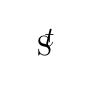
\begin{tikzpicture}[baseline=(top.base)]
                    \Tree [.\node(top){S}; [.DP [.D das ] [.NP essen ] ] [.VP $t$ ] ]
                \end{tikzpicture}
            \ex \begin{tikzpicture}[baseline=(top.base)]
                    \Tree [.\node(top){S\,^{{\color{red}\mathtt{?}}}_{{\color{red}?}} }; [.DP\,^{{\color{darkgray}\mathtt{FA\shortrightarrow}}}_{{\color{gray}e}} [.D\,^{{\color{darkgray}\mathtt{NN}}}_{{\color{gray}\langle \langle e,\, t\rangle,\, e\rangle}} das\,^{{\color{darkgray}\mathtt{TN_1}}}_{{\color{gray}\langle \langle e,\, t\rangle,\, e\rangle}} ] [.NP\,^{{\color{darkgray}\mathtt{NN}}}_{{\color{gray}\langle e,\, t\rangle}} essen\,^{{\color{darkgray}\mathtt{TN_1}}}_{{\color{gray}\langle e,\, t\rangle}} ] ] [.VP\,^{{\color{darkgray}\mathtt{NN}}}_{{\color{gray}e}} $t$\,^{{\color{darkgray}\mathtt{TN_2}}}_{{\color{gray}e}} ] ]
                \end{tikzpicture}
        \end{xlist}
    \end{exe}

\begin{exe}
    \ex Peter hits Peter.\hfill\textit{\footnotesize $4/15$ iterations, 0.26ms}
        \begin{xlist}
            % input string: "[.S [.NP [.N Peter ] ] [.VP [.V hits ] [.NP [.N Peter ] ] ] ]"
            \ex \begin{tikzpicture}[baseline=(top.base)]
                    \Tree [.\node(top){S}; [.NP [.N Peter ] ] [.VP [.V hits ] [.NP [.N Peter ] ] ] ]
                \end{tikzpicture}
            \ex \begin{tikzpicture}[baseline=(top.base)]
                    \Tree [.\node(top){S\,^{{\color{darkgray}\mathtt{FA\shortleftarrow}}}_{{\color{gray}t}} }; [.NP\,^{{\color{darkgray}\mathtt{NN}}}_{{\color{gray}e}} [.N\,^{{\color{darkgray}\mathtt{NN}}}_{{\color{gray}e}} Peter\,^{{\color{darkgray}\mathtt{TN_1}}}_{{\color{gray}e}} ] ] [.VP\,^{{\color{darkgray}\mathtt{FA\shortrightarrow}}}_{{\color{gray}\langle e,\, t\rangle}} [.V\,^{{\color{darkgray}\mathtt{NN}}}_{{\color{gray}\langle e,\, \langle e,\, t\rangle\rangle}} hits\,^{{\color{darkgray}\mathtt{TN_1}}}_{{\color{gray}\langle e,\, \langle e,\, t\rangle\rangle}} ] [.NP\,^{{\color{darkgray}\mathtt{NN}}}_{{\color{gray}e}} [.N\,^{{\color{darkgray}\mathtt{NN}}}_{{\color{gray}e}} Peter\,^{{\color{darkgray}\mathtt{TN_1}}}_{{\color{gray}e}} ] ] ] ]
                \end{tikzpicture}
        \end{xlist}
    \end{exe}

\begin{exe}
    \ex Alle Blumen sind stolz auf essen.\hfill\textit{\footnotesize $15/15$ iterations, 0.79ms}
        \begin{xlist}
            % input string: "[.S [.NP^1 [.Q alle ] [.N^1 Blumen ] ] [.VP [.V sind ] [.AP [.A stolz ] [.PP [.P auf ] [.NP^2 [.N^2 essen ] ] ] ] ] ]"
            \ex \begin{tikzpicture}[baseline=(top.base)]
                    \Tree [.\node(top){S}; [.NP [.Q alle ] [.N Blumen ] ] [.VP [.V sind ] [.AP [.A stolz ] [.PP [.P auf ] [.NP [.N essen ] ] ] ] ] ]
                \end{tikzpicture}
            \ex \begin{tikzpicture}[baseline=(top.base)]
                    \Tree [.\node(top){S\,^{{\color{red}\mathtt{?}}}_{{\color{red}?}} }; [.NP\,^{{\color{darkgray}\mathtt{FA\shortrightarrow}}}_{{\color{gray}\langle \langle e,\, t\rangle,\, t\rangle}} [.Q\,^{{\color{darkgray}\mathtt{NN}}}_{{\color{gray}\langle \langle e,\, t\rangle,\, \langle \langle e,\, t\rangle,\, t\rangle\rangle}} alle\,^{{\color{darkgray}\mathtt{TN_1}}}_{{\color{gray}\langle \langle e,\, t\rangle,\, \langle \langle e,\, t\rangle,\, t\rangle\rangle}} ] [.N\,^{{\color{darkgray}\mathtt{NN}}}_{{\color{gray}\langle e,\, t\rangle}} Blumen\,^{{\color{darkgray}\mathtt{TN_1}}}_{{\color{gray}\langle e,\, t\rangle}} ] ] [.VP\,^{{\color{darkgray}\mathtt{NN}}}_{{\color{red}?}} [.V\,^{{\color{darkgray}\mathtt{NN}}}_{{\color{gray}-}} sind\,^{{\color{darkgray}\mathtt{-}}}_{{\color{gray}-}} ] [.AP\,^{{\color{red}\mathtt{?}}}_{{\color{red}?}} [.A\,^{{\color{darkgray}\mathtt{NN}}}_{{\color{gray}\langle e,\, \langle e,\, t\rangle\rangle}} stolz\,^{{\color{darkgray}\mathtt{TN_1}}}_{{\color{gray}\langle e,\, \langle e,\, t\rangle\rangle}} ] [.PP\,^{{\color{darkgray}\mathtt{NN}}}_{{\color{gray}\langle e,\, t\rangle}} [.P\,^{{\color{darkgray}\mathtt{NN}}}_{{\color{gray}-}} auf\,^{{\color{darkgray}\mathtt{-}}}_{{\color{gray}-}} ] [.NP\,^{{\color{darkgray}\mathtt{NN}}}_{{\color{gray}\langle e,\, t\rangle}} [.N\,^{{\color{darkgray}\mathtt{NN}}}_{{\color{gray}\langle e,\, t\rangle}} essen\,^{{\color{darkgray}\mathtt{TN_1}}}_{{\color{gray}\langle e,\, t\rangle}} ] ] ] ] ] ]
                \end{tikzpicture}
        \end{xlist}
    \end{exe}

\begin{exe}
    \ex Der Junge der_{RP} wo die Fee aus Nimmerland belästigt fliegt.\hfill\textit{\footnotesize $9/15$ iterations, 1.49ms}
        \begin{xlist}
            % input string: "[.S [.DP [.D der ] [.NP [.N$''$ [.N$'$ [.N Junge ] ] [.CP [.DP der_{RP} ] [.C$'$ [.C wo ] [.S$'$ [.$t$_1 ] [.VP [.DP [.D die ] [.NP [.N$''$ [.N$'$ [.N Fee ] ] [.PP [.P aus ] [.DP Nimmerland ] ] ] ] ]  [.V belästigt ] ] ] ] ] ] ] ]  [.VP [.V fliegt ] ] ]"
            \ex \begin{tikzpicture}[baseline=(top.base)]
                    \Tree [.\node(top){S}; [.DP [.D der ] [.NP [.N$''$ [.N$'$ [.N Junge ] ] [.CP [.DP der_{RP} ] [.C$'$ [.C wo ] [.S$'$ [.$t$_1 ] [.VP [.DP [.D die ] [.NP [.N$''$ [.N$'$ [.N Fee ] ] [.PP [.P aus ] [.DP Nimmerland ] ] ] ] ]  [.V belästigt ] ] ] ] ] ] ] ]  [.VP [.V fliegt ] ] ]
                \end{tikzpicture}
            \ex \begin{tikzpicture}[baseline=(top.base)]
                    \Tree [.\node(top){S\,^{{\color{darkgray}\mathtt{FA\shortleftarrow}}}_{{\color{gray}t}} }; [.DP\,^{{\color{darkgray}\mathtt{FA\shortrightarrow}}}_{{\color{gray}e}} [.D\,^{{\color{darkgray}\mathtt{NN}}}_{{\color{gray}\langle \langle e,\, t\rangle,\, e\rangle}} der\,^{{\color{darkgray}\mathtt{TN_1}}}_{{\color{gray}\langle \langle e,\, t\rangle,\, e\rangle}} ] [.NP\,^{{\color{darkgray}\mathtt{NN}}}_{{\color{gray}\langle e,\, t\rangle}} [.N$''$\,^{{\color{darkgray}\mathtt{PM}}}_{{\color{gray}\langle e,\, t\rangle}} [.N$'$\,^{{\color{darkgray}\mathtt{NN}}}_{{\color{gray}\langle e,\, t\rangle}} [.N\,^{{\color{darkgray}\mathtt{NN}}}_{{\color{gray}\langle e,\, t\rangle}} Junge\,^{{\color{darkgray}\mathtt{TN_1}}}_{{\color{gray}\langle e,\, t\rangle}} ] ] [.CP\,^{{\color{darkgray}\mathtt{PA}}}_{{\color{gray}\langle e,\, t\rangle}} [.DP\,^{{\color{darkgray}\mathtt{NN}}}_{{\color{gray}-}} der_{RP}\,^{{\color{darkgray}\mathtt{-}}}_{{\color{gray}-}} ] [.C$'$\,^{{\color{darkgray}\mathtt{NN}}}_{{\color{gray}t}} [.C\,^{{\color{darkgray}\mathtt{NN}}}_{{\color{gray}-}} wo\,^{{\color{darkgray}\mathtt{-}}}_{{\color{gray}-}} ] [.S$'$\,^{{\color{darkgray}\mathtt{FA\shortleftarrow}}}_{{\color{gray}t}} [.$t$\,^{{\color{darkgray}\mathtt{TN_2}}}_{{\color{gray}e}} ] [.VP\,^{{\color{darkgray}\mathtt{FA\shortleftarrow}}}_{{\color{gray}\langle e,\, t\rangle}} [.DP\,^{{\color{darkgray}\mathtt{FA\shortrightarrow}}}_{{\color{gray}e}} [.D\,^{{\color{darkgray}\mathtt{NN}}}_{{\color{gray}\langle \langle e,\, t\rangle,\, e\rangle}} die\,^{{\color{darkgray}\mathtt{TN_1}}}_{{\color{gray}\langle \langle e,\, t\rangle,\, e\rangle}} ] [.NP\,^{{\color{darkgray}\mathtt{NN}}}_{{\color{gray}\langle e,\, t\rangle}} [.N$''$\,^{{\color{darkgray}\mathtt{PM}}}_{{\color{gray}\langle e,\, t\rangle}} [.N$'$\,^{{\color{darkgray}\mathtt{NN}}}_{{\color{gray}\langle e,\, t\rangle}} [.N\,^{{\color{darkgray}\mathtt{NN}}}_{{\color{gray}\langle e,\, t\rangle}} Fee\,^{{\color{darkgray}\mathtt{TN_1}}}_{{\color{gray}\langle e,\, t\rangle}} ] ] [.PP\,^{{\color{darkgray}\mathtt{FA\shortrightarrow}}}_{{\color{gray}\langle e,\, t\rangle}} [.P\,^{{\color{darkgray}\mathtt{NN}}}_{{\color{gray}\langle e,\, \langle e,\, t\rangle\rangle}} aus\,^{{\color{darkgray}\mathtt{TN_1}}}_{{\color{gray}\langle e,\, \langle e,\, t\rangle\rangle}} ] [.DP\,^{{\color{darkgray}\mathtt{NN}}}_{{\color{gray}e}} Nimmerland\,^{{\color{darkgray}\mathtt{TN_1}}}_{{\color{gray}e}} ] ] ] ] ]  [.V\,^{{\color{darkgray}\mathtt{NN}}}_{{\color{gray}\langle e,\, \langle e,\, t\rangle\rangle}} belästigt\,^{{\color{darkgray}\mathtt{TN_1}}}_{{\color{gray}\langle e,\, \langle e,\, t\rangle\rangle}} ] ] ] ] ] ] ] ]  [.VP\,^{{\color{darkgray}\mathtt{NN}}}_{{\color{gray}\langle e,\, t\rangle}} [.V\,^{{\color{darkgray}\mathtt{NN}}}_{{\color{gray}\langle e,\, t\rangle}} fliegt\,^{{\color{darkgray}\mathtt{TN_1}}}_{{\color{gray}\langle e,\, t\rangle}} ] ] ]
                \end{tikzpicture}
        \end{xlist}
    \end{exe}

